\documentclass[onecolumn]{article}
\usepackage{xurl}
\usepackage{graphicx}
\title{Medical Imaging Computing Assignment 2}

\author{Suneet Tipirneni}

\begin{document}
\maketitle
\section{Code}
Code can be found at \url{https://github.com/suneettipirneni/med-proj-2}
\section{Dataset Visualization via ITK-SNAP}

Below is a demo of the a visualization I took from the dataset using ITK-SNAP:

\begin{figure}[htpb]
	\centering
	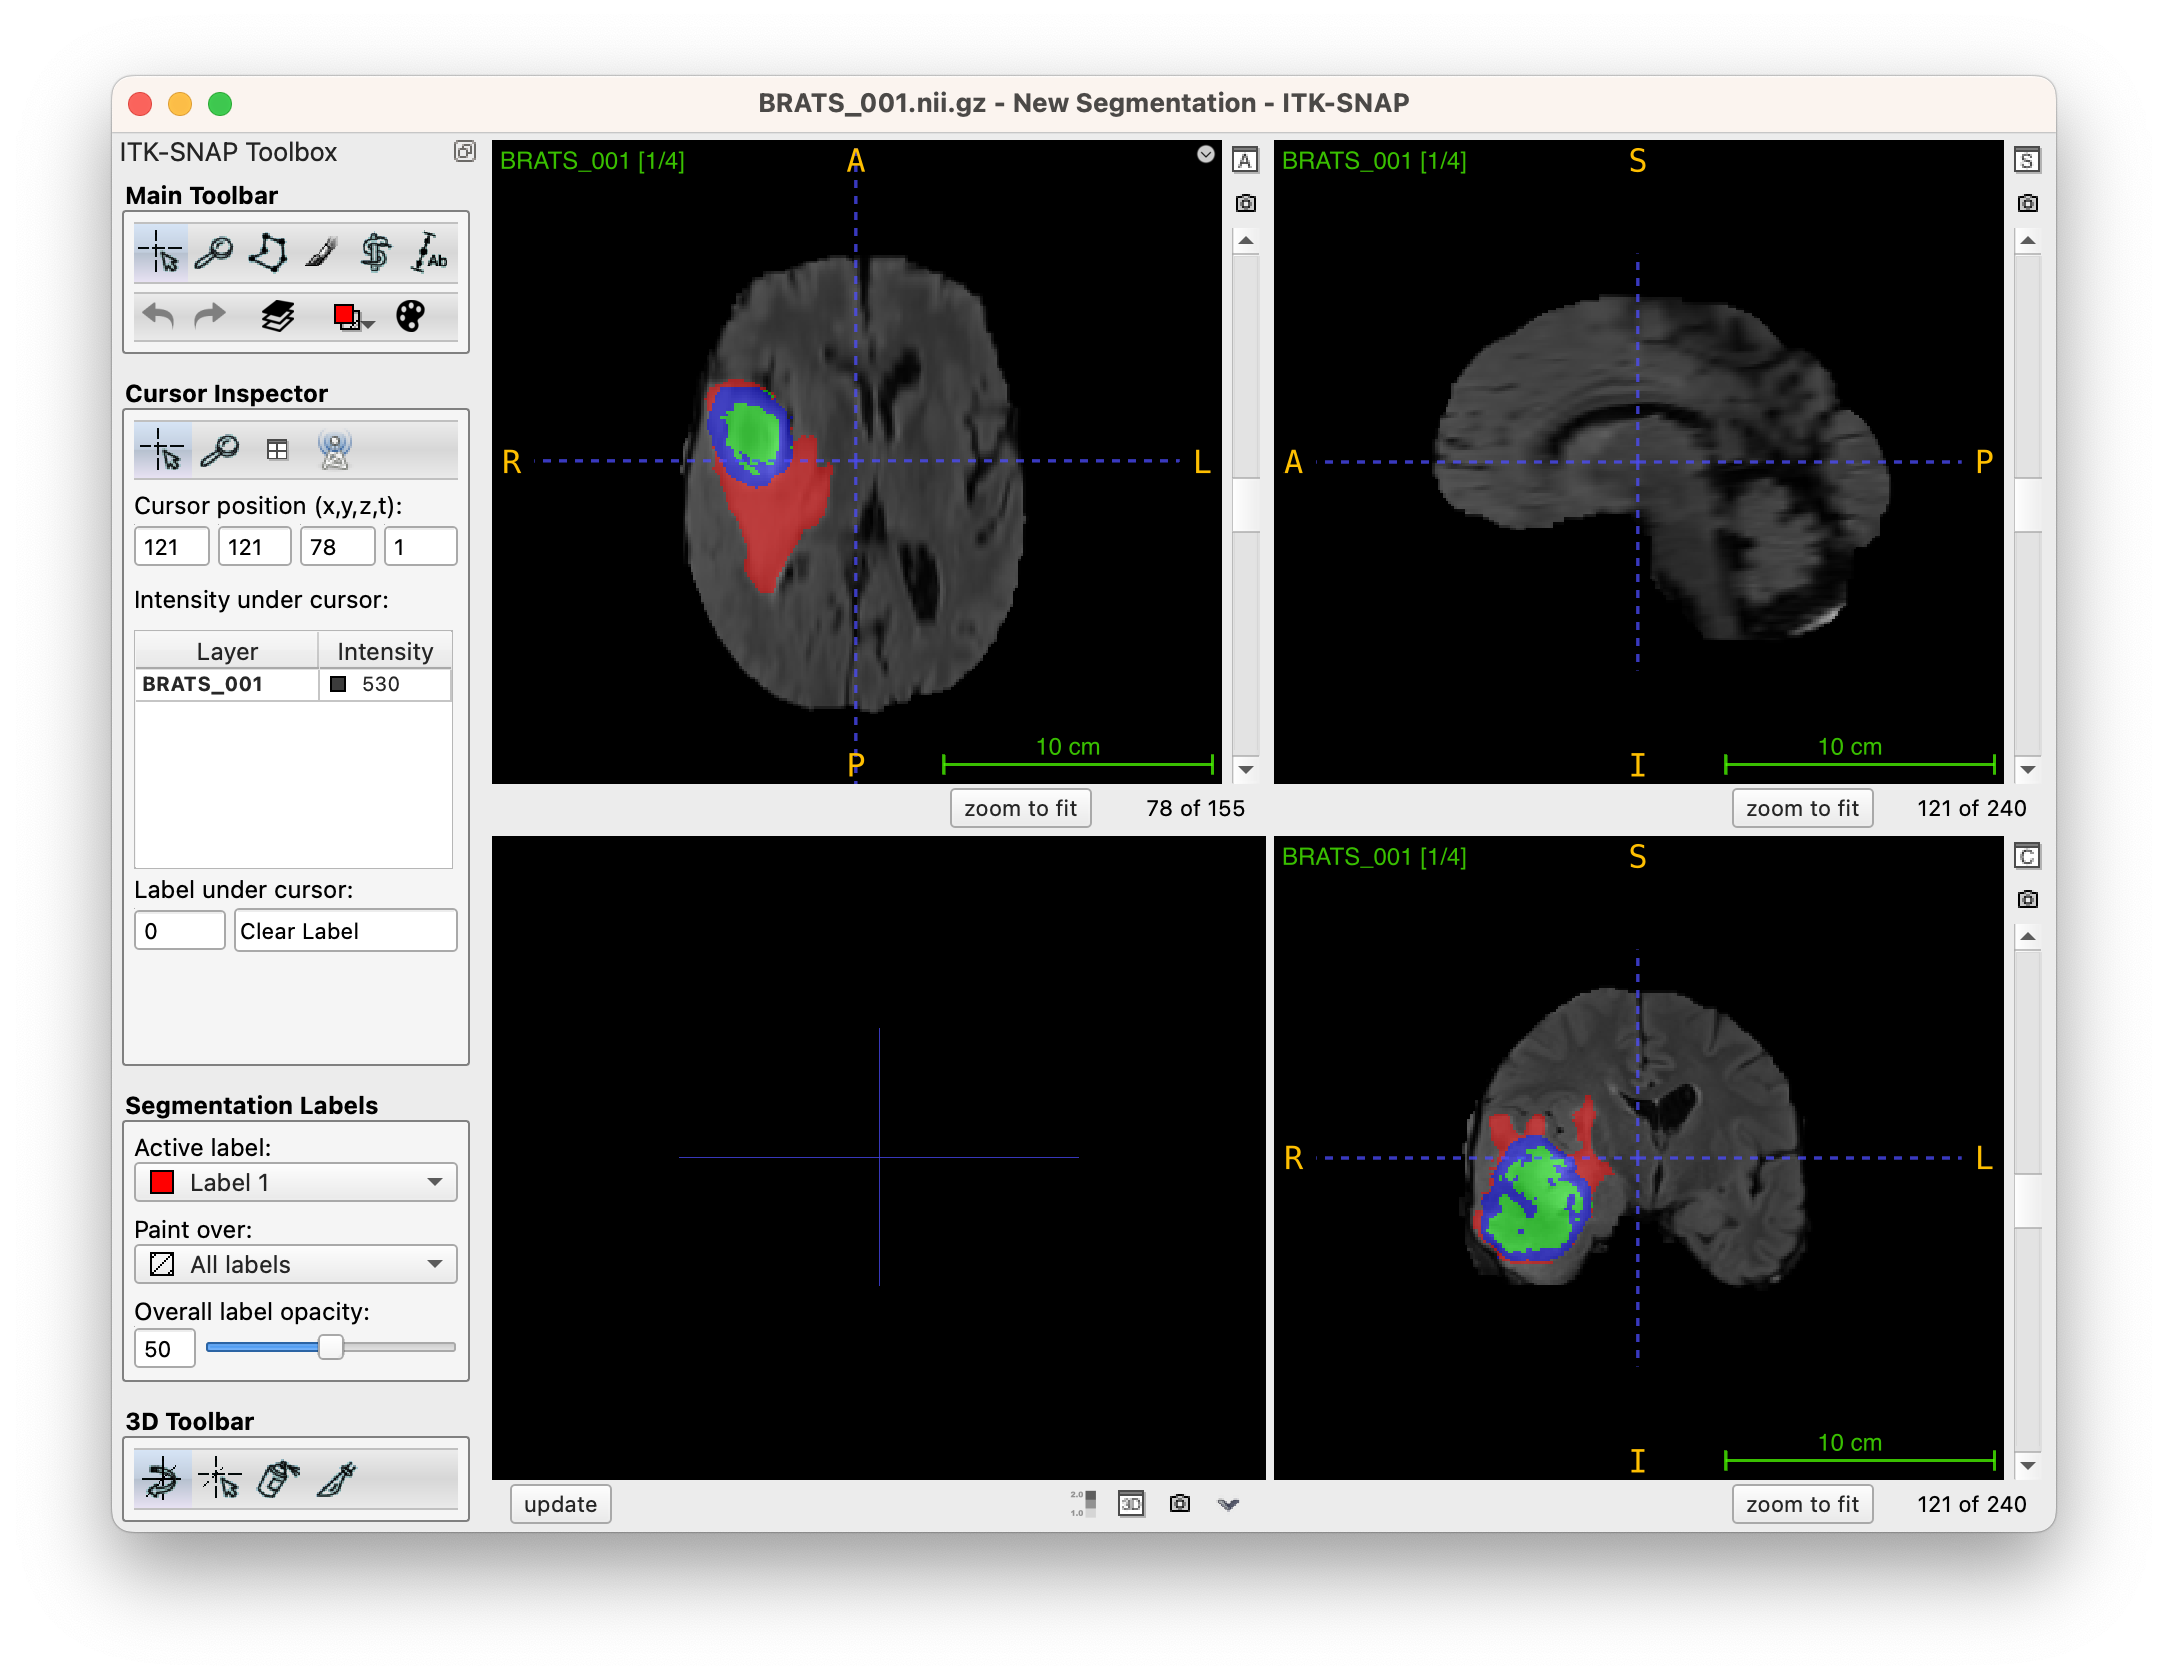
\includegraphics[width=0.8\textwidth]{imgs/itk-snap.png}
	\caption{A screenshot of the ITK-SNAP visualiation of a sample from the dataset.}
\end{figure}

\section{Implementation}

My implementation for this model is adapted from \cite{monaitutorial}. The core change from that tutorial to my code is that I use a MONAI's UNETR class for 3d image segmentation. I choose UNETR as it has achvied really good results with 3d image segmentation \cite{hatamizadeh2021unetr}. I choose to use the same image transformations found in \cite{monaitutorial} however, I changed the crop size of the images to $128\times 128 \times 128$. My reasoning for this was it improved the training time by a lot from the default image size of $224 \times 224 \times 155$. This dimension specifically, was found in the SWIN UNETR tutorial \cite{githubTutorialsswin_unetr_brats21_segmentation_3dipynbMain}. In hindsight I later realized that the square shape was more specific to SWIN model patches, however this didn't seem to have much effect on my results. In addition to using UNETR, I used an additional metric to measure the Hausdoff distance. This was provided via \cite{githubGitHubLolimedpy}. An issue however was with the calulations that this library did. It did not accept all-0 ground truth masks. As a result during evaluation I had to the filter out any masks that were all zeroes in order for the calculation to work properly. In addition, my model uses 5-fold cross validation based on the scikit learn $KFold$ utility \cite{githubMachinelearningarticleshowtousekfoldcrossvalidationwithpytorchmdMain}. I ran the model for 25 epochs, where each fold used 5 epochs. The reason my epoch count is low is the training took a very long time. 

\section{Accurracies}

The model achieved an accuracy around 65\%. Which is sub-par. However upon further inspection this is most likely due to the fact that the model did not train for long enough. The losses and scores were improving at the 25 epoch cutoff so perhaps it would do much better with more training. 

\begin{table}[!ht] \label{tab:1}
\begin{tabular}{lll}
Fold & Dice Average & Hausdoff Distance Average \\
1    & 0.59         & 45.6                      \\
2    & 0.61         & 36.2                      \\
3    & 0.64         & 32.7                      \\
4    & 0.67         & 33.8                      \\
5    & 0.65         & 37.514                    \\
All  & 0.63         & 37.16                     \\
\end{tabular}
\caption{Average score for each fold in training}
\end{table}

\newpage

The calculation of these individual accuracies uses the code from \cite{training}. 

\section{Qualitative Analysis}

Using the visualization code from \cite{monaitutorial} the predictions of the model are produced along with the ground truth and the input data. Personally, I think the results here are quite satisfactory both the predicted and ground truth masks looks very close.

\begin{figure*}[!ht]
	\centering
	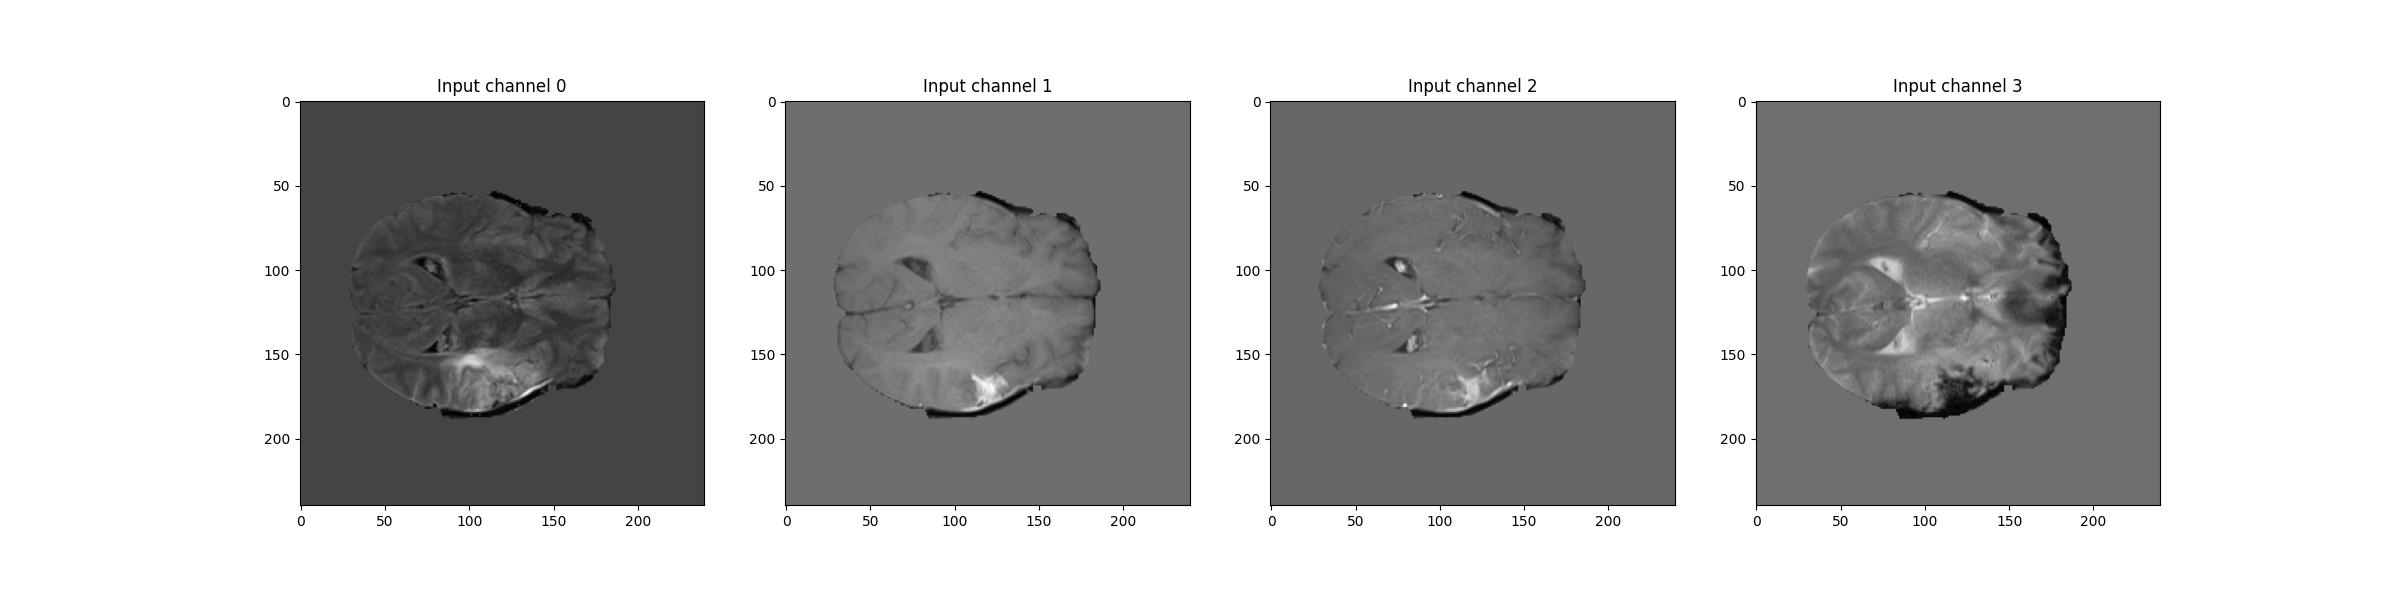
\includegraphics[width=0.9\textwidth]{imgs/inputs1.png}
	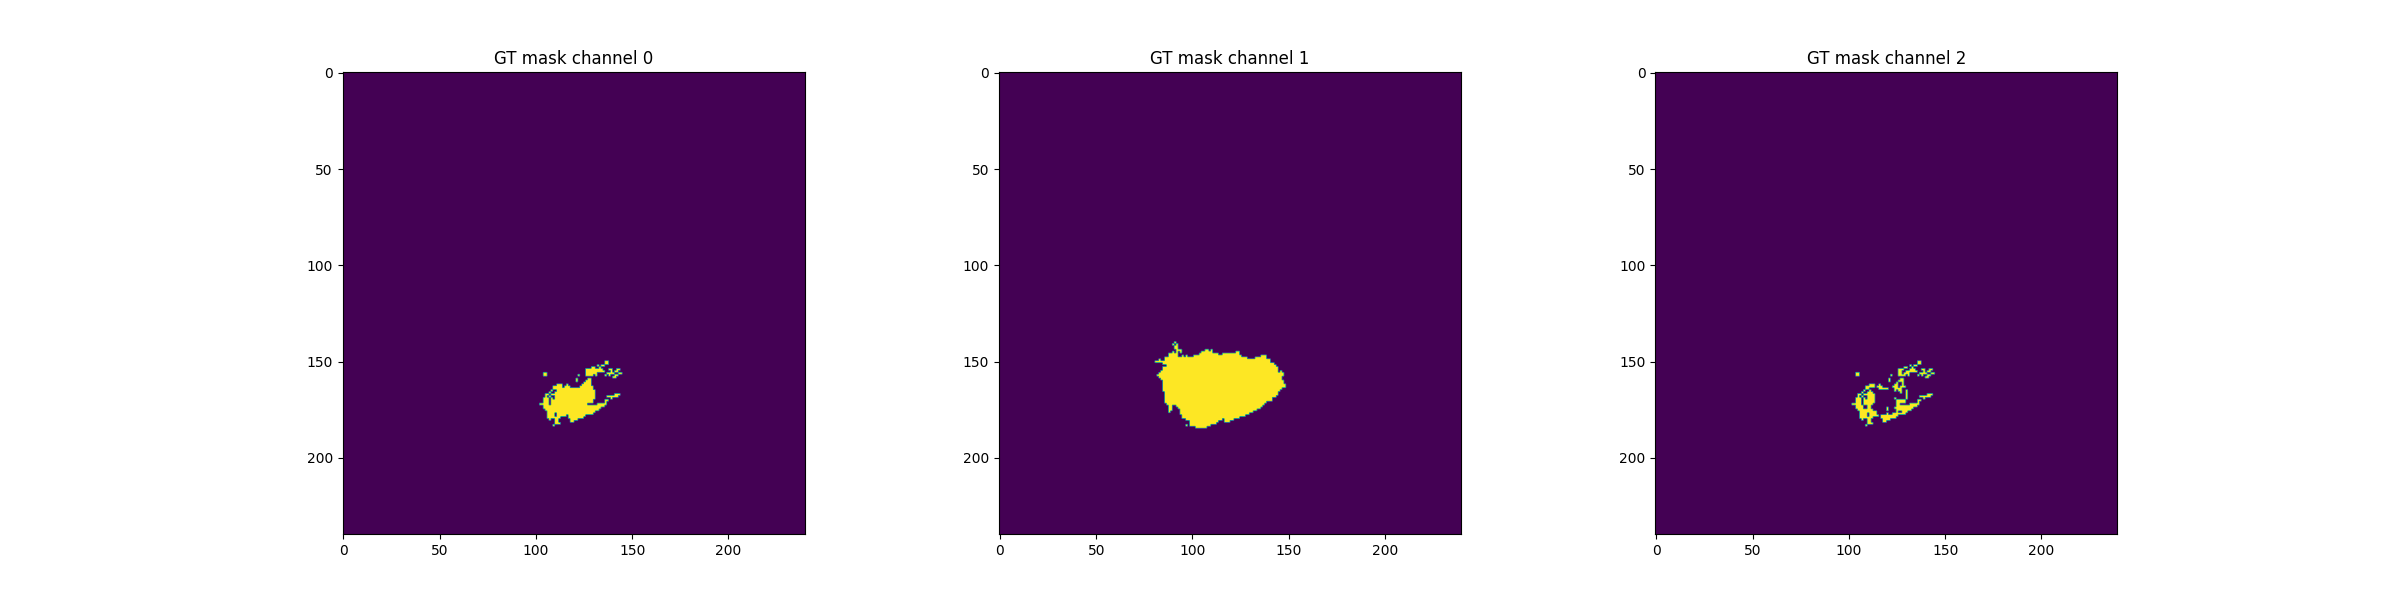
\includegraphics[width=0.9\textwidth]{imgs/gt1.png}
	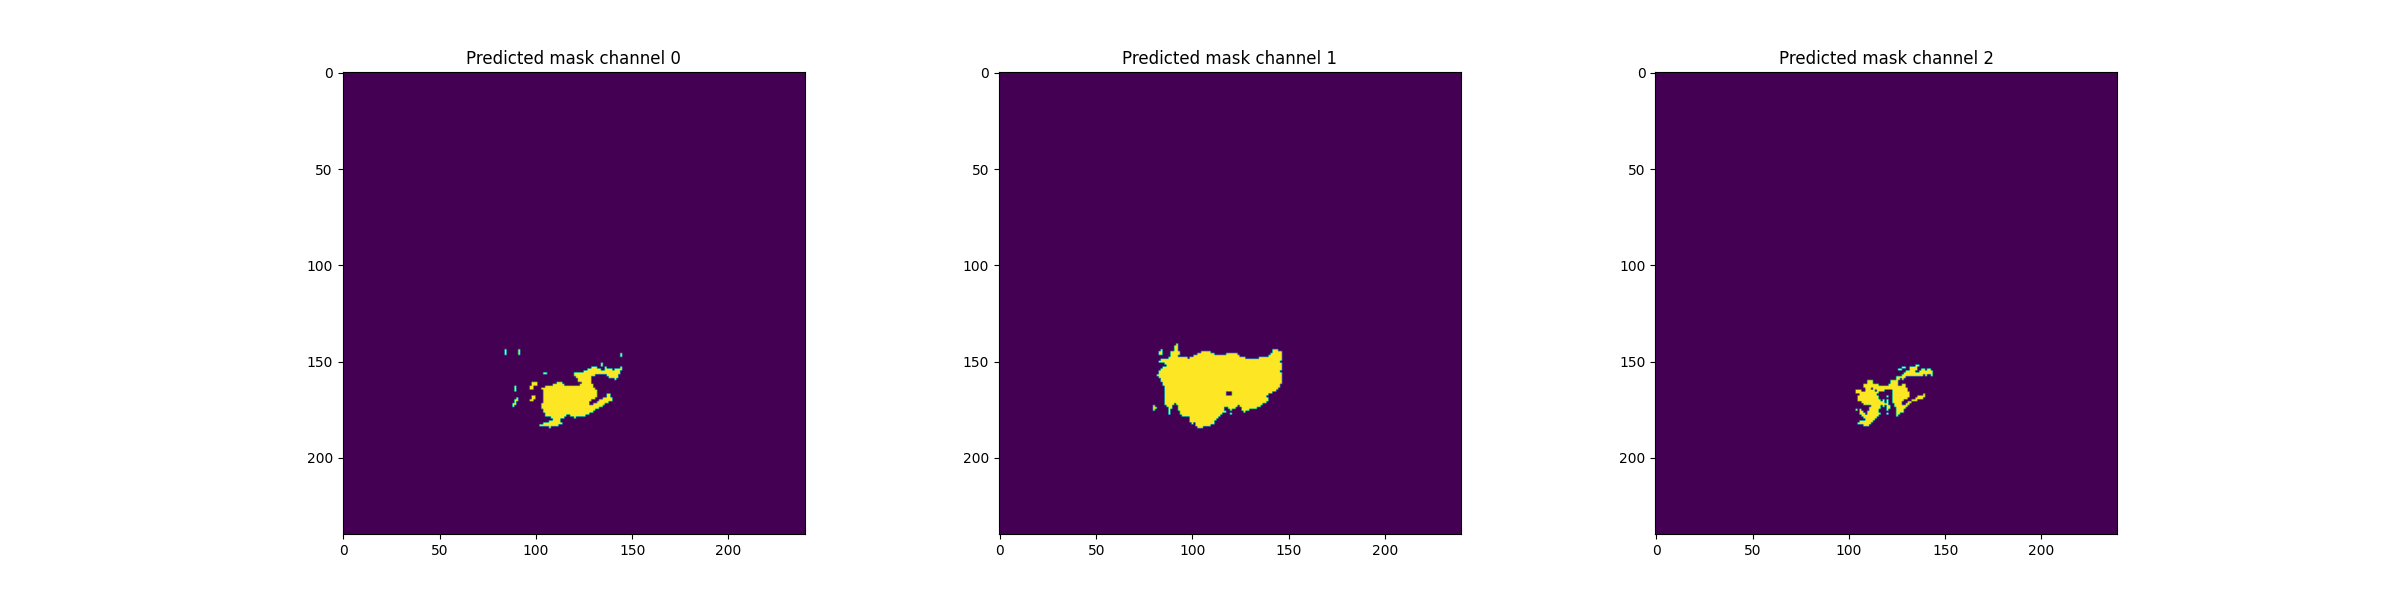
\includegraphics[width=0.9\textwidth]{imgs/pred1.png}
	\caption{First qualitative sample from the model, the first row is the input, the second is the ground truth masks, and the third row is the predicted masks.}
	\label{fig:res2}
\end{figure*}

\begin{figure*}[!ht]
	\centering
	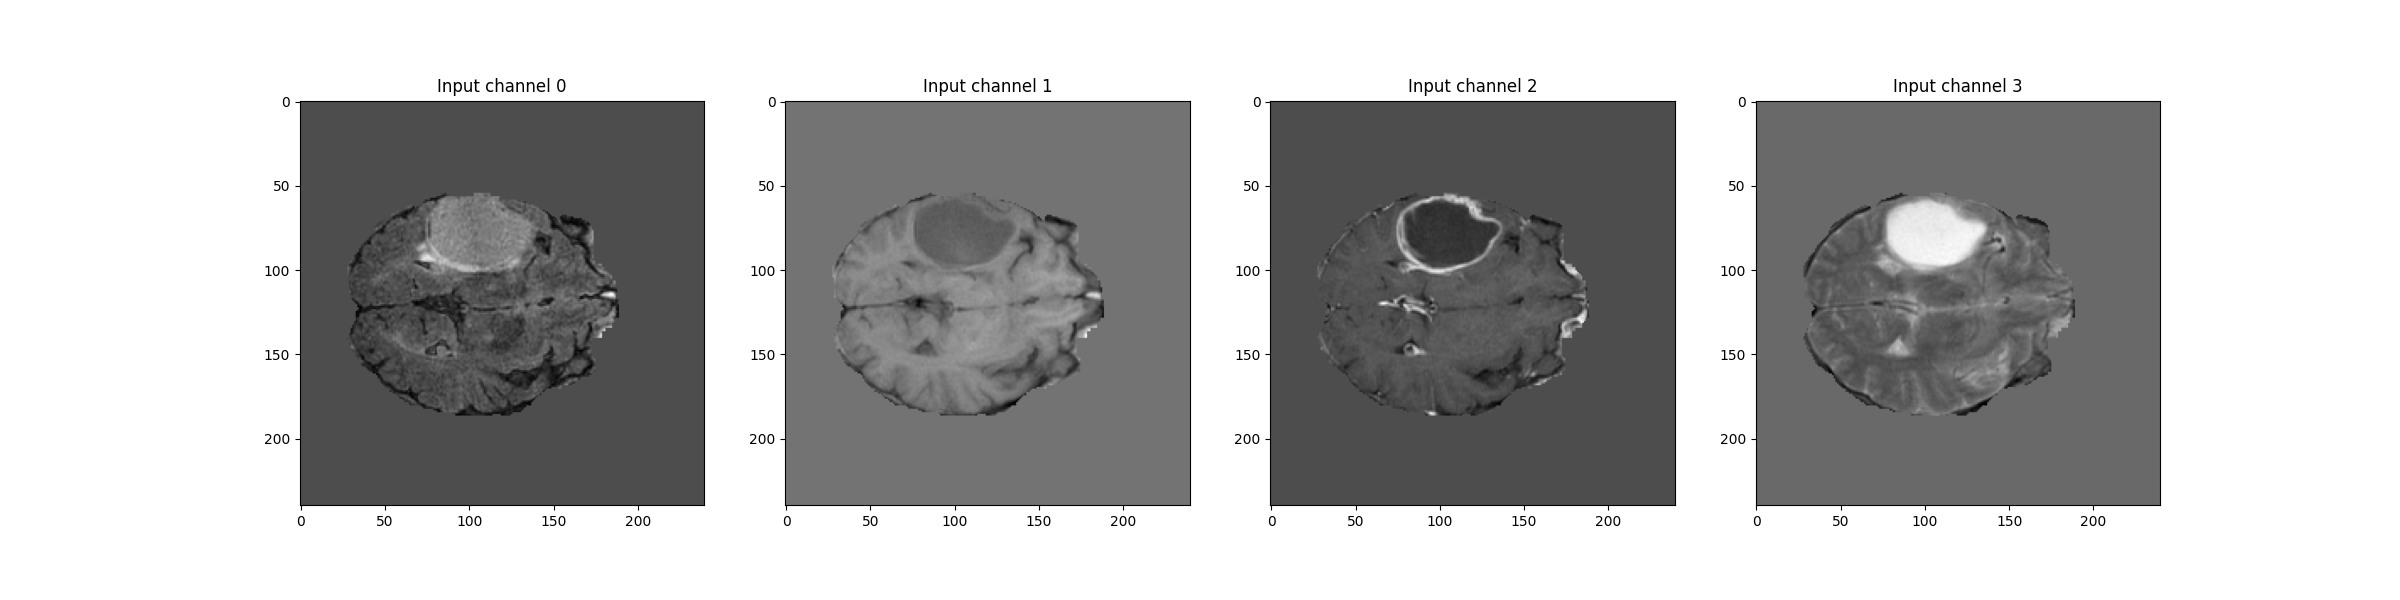
\includegraphics[width=0.9\textwidth]{imgs/inputs2.png}
	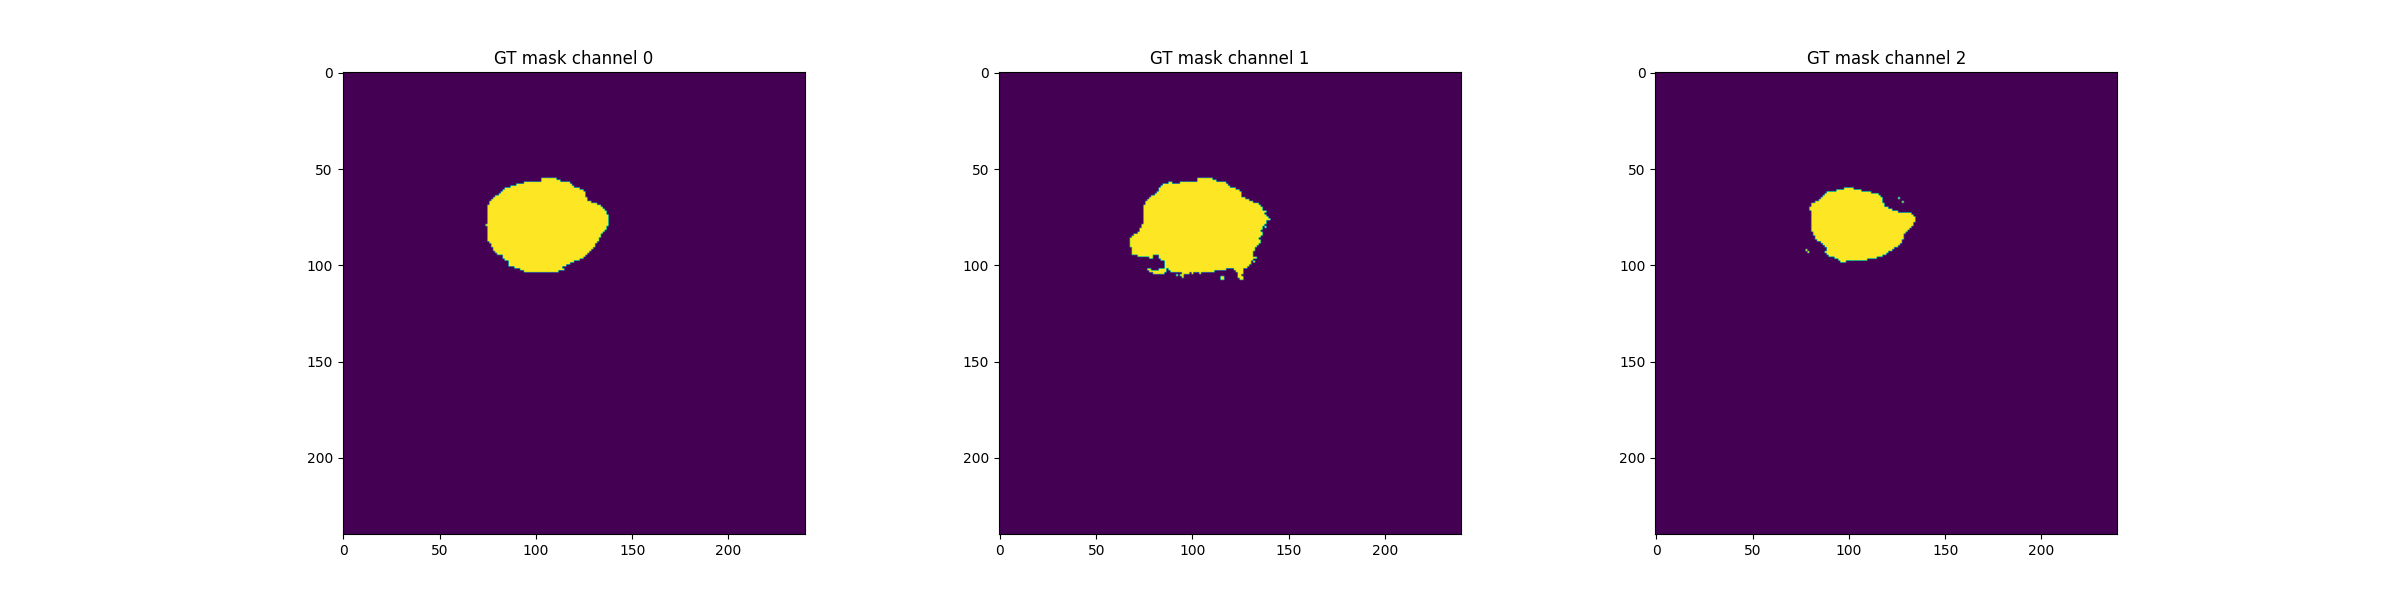
\includegraphics[width=0.9\textwidth]{imgs/gt2.png}
	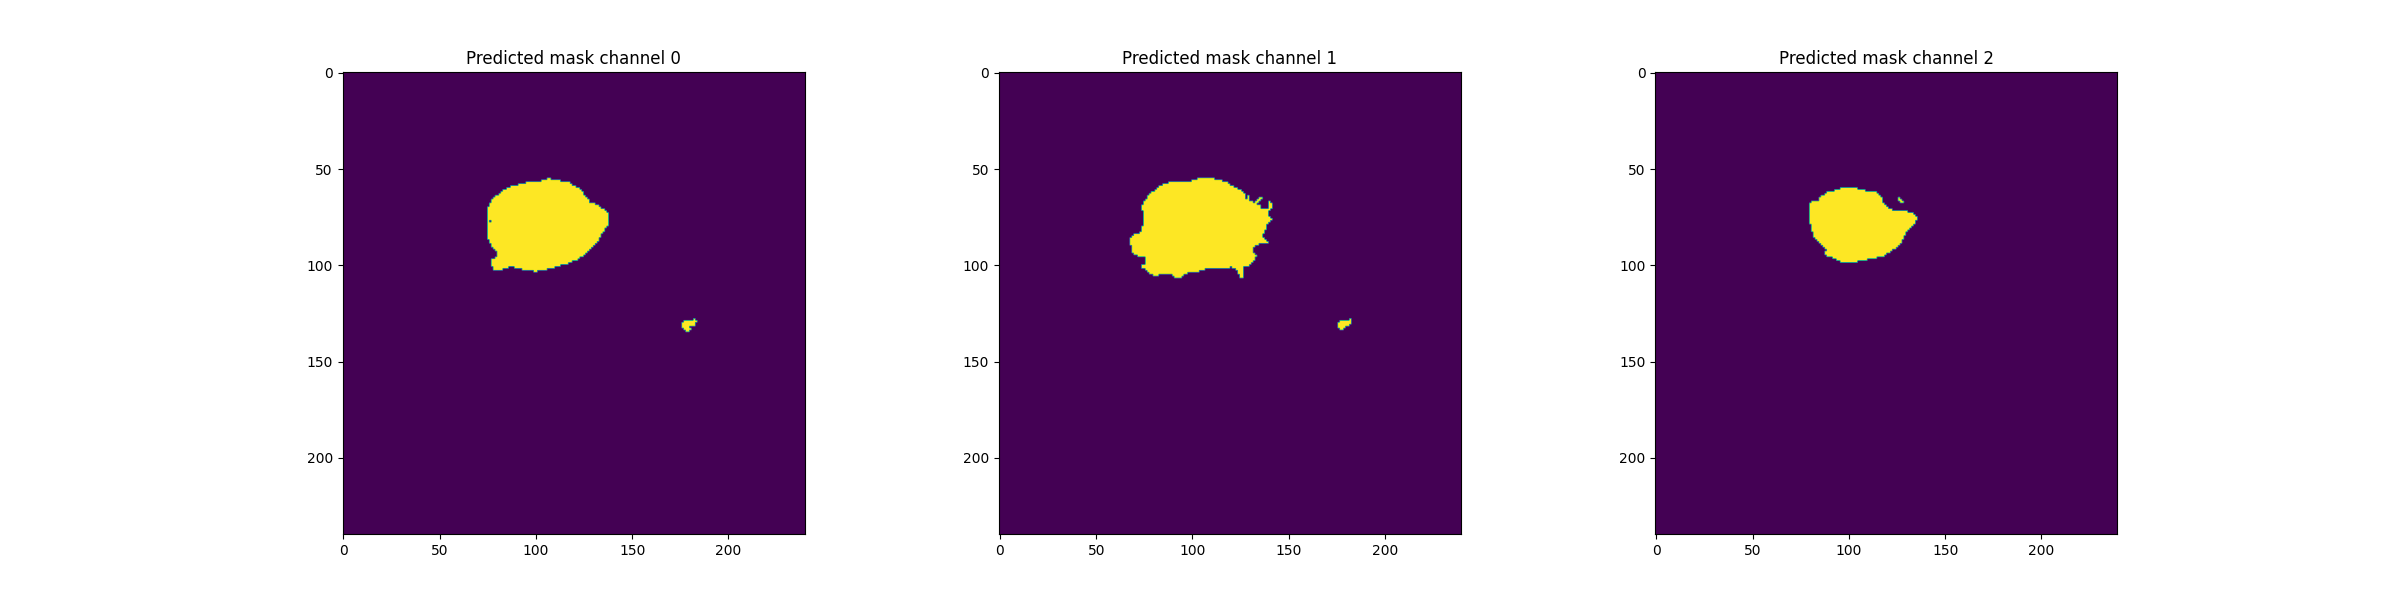
\includegraphics[width=0.9\textwidth]{imgs/pred2.png}
	\caption{Another visualization of the predictions, this follows the same layout described in figure 2.}
	\label{fig:}
\end{figure*}

\newpage

\bibliographystyle{acm}
\bibliography{references}

	
\end{document}
